\documentclass[11pt]{article}
\usepackage[a4paper,margin=25mm]{geometry}
\usepackage{amsmath,amssymb,amsthm,booktabs,tikz,hyperref}
\hypersetup{colorlinks=true,linkcolor=blue,urlcolor=blue,citecolor=blue}
\newtheorem{theorem}{Theorem}
\newtheorem{lemma}{Lemma}
\newcommand{\DS}{\mathrm{DS}}
\newcommand{\E}{\mathcal E_{\DS}}
\title{A connected graph with integer diminished Sombor energy}
\author{Principia Math In Progress}
\date{29 September 2026}
\begin{document}
\maketitle
\begin{abstract}
We construct a connected simple bipartite graph on \(77\) vertices with
diminished Sombor energy \(72\), disproving Movahedi's nonintegrality
conjecture. Its six nonzero eigenvalues are
\(\pm10,\ \pm(13+\sqrt{29}),\ \pm(13-\sqrt{29})\).
The construction also gives connected counterexamples of arbitrarily
large minimum degree.
\end{abstract}

\section*{Task 1. The conjecture and its resolution}
For a finite simple graph \(G\), let \(d_v\) be the degree of \(v\). Its
diminished Sombor matrix and energy are
\[
 (M_{\DS}(G))_{uv}=
 \begin{cases}
 \dfrac{\sqrt{d_u^2+d_v^2}}{d_u+d_v},&uv\in E(G),\\
 0,&uv\notin E(G),
 \end{cases}
 \qquad
 \E(G)=\sum_{\lambda\in\operatorname{Spec}M_{\DS}(G)}|\lambda|,
\]
where eigenvalues are counted with multiplicity. Conjecture 5.1 of
\cite{movahedi}, p.~19, asserts that this energy is never an integer.
This is the question recorded as
\href{https://mathdb.com/p/369710}{MathDB 369710}.
The following counterexample is connected and has minimum degree \(21\).

\begin{theorem}\label{thm:main}
There is a connected simple bipartite graph \(G\) with \(77\) vertices,
\(980\) edges, \(28\) vertices of degree \(21\), and \(49\) vertices of
degree \(28\), such that
\[
 \operatorname{Spec}M_{\DS}(G)
 =\{10,-10,\ 13+\sqrt{29},-13-\sqrt{29},\
       13-\sqrt{29},-13+\sqrt{29},\ 0^{(71)}\}.
\]
In particular, \(\E(G)=72\).
\end{theorem}

\paragraph{An eleven-vertex graph.}
Define \(H\) using disjoint independent vertex classes
\[
 |A_1|=|A_2|=|B_1|=|B_2|=|C|=2,\qquad |D|=1.
\]
Put in every edge between each of the following six pairs of classes,
and put in no other edges:
\[
 A_1B_1,\quad A_2B_2,\quad A_1D,\quad A_2D,\quad CB_1,\quad CB_2.
\]
Thus \(H\) is the blowup of a six-cycle with five classes of size two
and one class of size one. Its bipartition is
\((A_1\cup A_2\cup C,\ B_1\cup B_2\cup D)\).
It is connected, has \(20\) edges, and has degree \(3\) on \(A_1\cup A_2\)
and degree \(4\) on all other vertices.
\begin{center}
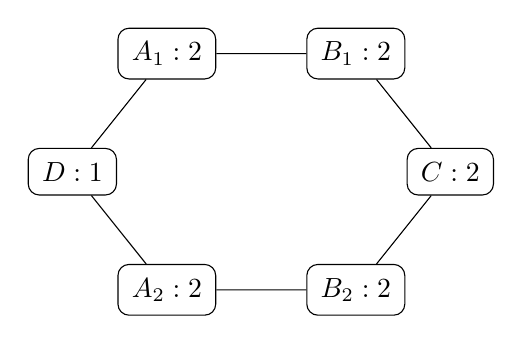
\begin{tikzpicture}[every node/.style={draw,rounded corners,inner sep=5pt}]
\node (a1) at (0,1.5) {\(A_1:2\)};
\node (b1) at (2.4,1.5) {\(B_1:2\)};
\node (c) at (3.6,0) {\(C:2\)};
\node (b2) at (2.4,-1.5) {\(B_2:2\)};
\node (a2) at (0,-1.5) {\(A_2:2\)};
\node (d) at (-1.2,0) {\(D:1\)};
\draw (a1)--(b1)--(c)--(b2)--(a2)--(d)--(a1);
\end{tikzpicture}

\small Each drawn edge denotes all edges between its two independent classes.
\end{center}

\section*{Exact spectrum of the base graph}
The diminished Sombor weights on the degree pairs \((3,4)\) and \((4,4)\)
are, respectively,
\[
 u=\frac57,\qquad w=\frac1{\sqrt2}.
\]
Order the two sides of the bipartition as above, and write
\(M_{\DS}(H)=\left(\begin{smallmatrix}0&B\\B^{\mathsf T}&0\end{smallmatrix}\right)\).
If \(J_2\) is the two-by-two all-ones matrix and
\(\mathbf1_2=(1,1)^{\mathsf T}\), then
\[
 B=\begin{pmatrix}
 uJ_2&0&u\mathbf1_2\\
 0&uJ_2&u\mathbf1_2\\
 wJ_2&wJ_2&0
 \end{pmatrix}.
\]
Vectors summing to zero inside a vertex class are annihilated by the
appropriate block. On the subspaces of vectors constant on classes,
use the normalized indicator vectors of the classes. The resulting
three-by-three matrix is
\[
 R=\begin{pmatrix}
 10/7&0&5\sqrt2/7\\
 0&10/7&5\sqrt2/7\\
 \sqrt2&\sqrt2&0
 \end{pmatrix}.
\]
Consequently the nonzero singular values of \(B\) are those of \(R\).
Replacing the first two coordinates on both sides by their normalized
difference and sum gives the orthogonal block decomposition
\[
 R\ \sim\ \frac{10}{7}\ \oplus\ T,
 \qquad
 T=\begin{pmatrix}10/7&10/7\\2&0\end{pmatrix}.
\]
Let \(s_+\ge s_->0\) be the singular values of \(T\).
The trace and determinant identities give
\[
 s_+^2+s_-^2=\operatorname{tr}(TT^{\mathsf T})=\frac{396}{49},
 \qquad s_+s_-=|\det T|=\frac{20}{7}.
\]
It follows that
\[
 (s_++s_-)^2=\frac{676}{49},\qquad
 s_++s_-=\frac{26}{7},\qquad
 s_\pm=\frac{13\pm\sqrt{29}}7.
\]
Both values are positive because \(13^2>29\). Since \(B\) has rank three,
the standard symmetric bipartite block form gives
\[
 \operatorname{Spec}M_{\DS}(H)
 =\left\{\pm\frac{10}7,\
          \pm\frac{13+\sqrt{29}}7,\
          \pm\frac{13-\sqrt{29}}7,\ 0^{(5)}\right\}.
\]
In particular,
\[
 \E(H)=2\left(\frac{10}7+\frac{26}7\right)=\frac{72}7.
\]

\section*{Blowup and integer energy}
\begin{lemma}\label{lem:blowup}
For a positive integer \(r\), replace each vertex of a simple graph \(F\)
by \(r\) independent vertices, and each edge by all \(r^2\) cross edges.
Denote the resulting graph by \(F^{(r)}\). Then
\[
 M_{\DS}(F^{(r)})=M_{\DS}(F)\otimes J_r,\qquad
 \E(F^{(r)})=r\,\E(F).
\]
\end{lemma}
\begin{proof}
Each new vertex corresponding to \(v\) has degree \(rd_v\). On an edge
the weight is unchanged, since
\[
 \frac{\sqrt{(rd_u)^2+(rd_v)^2}}{rd_u+rd_v}
 =\frac{\sqrt{d_u^2+d_v^2}}{d_u+d_v}.
\]
This proves the matrix identity. The eigenvalues of \(J_r\) are \(r\)
once and zero \(r-1\) times. The tensor-product eigenvalues now give the
energy identity.
\end{proof}

\begin{proof}[Proof of Theorem \ref{thm:main}]
Take \(G=H^{(7)}\). Equivalently, in the six-class construction replace
each class of size two by a class of size \(14\), and the singleton
class by a class of size \(7\). The graph is simple and bipartite.
It is connected: every path in \(H\) lifts between corresponding classes,
and two vertices in the same class have a common neighbor.
There are \(7\cdot11=77\) vertices and \(7^2\cdot20=980\) edges.
The \(4\cdot7=28\) vertices over \(A_1\cup A_2\) have degree \(21\);
the other \(7\cdot7=49\) vertices have degree \(28\).
Lemma \ref{lem:blowup} multiplies the six nonzero eigenvalues of \(H\)
by seven and supplies the other \(71\) zero eigenvalues.
Finally,
\[
 \E(G)=2\bigl(10+(13+\sqrt{29})+(13-\sqrt{29})\bigr)=72.
\]
\end{proof}

More generally, \(\E(H^{(r)})=72r/7\), which is an integer exactly when
\(7\mid r\). Thus \(H^{(7t)}\), for every integer \(t\ge1\), is a connected
counterexample with \(77t\) vertices, \(980t^2\) edges, minimum degree
\(21t\), and energy \(72t\).

\paragraph{Reproducible verification.}
The accompanying standard-library script independently constructs the
eleven- and seventy-seven-vertex graphs from their edges, checks the
degree-based weights in exact arithmetic, and verifies the spectrum by
matrix and Gram-matrix characteristic-polynomial calculations. For \(G\),
\[
 \det(xI-M_{\DS}(G))
   =x^{71}(x^2-100)(x^4-396x^2+19600).
\]
These finite checks supplement the symbolic proof above.

\section*{Four follow-up questions}
\paragraph{Task 2.} Determine the minimum order of a connected simple
graph with positive integer diminished Sombor energy.
\paragraph{Task 3.} Decide whether every tree with at least one edge
has irrational diminished Sombor energy.
\paragraph{Task 4.} Decide whether a simple graph can have odd integer
diminished Sombor energy.
\paragraph{Task 5.} Construct, or rule out, a connected graph with positive
integer diminished Sombor energy in which no two distinct vertices have
the same open neighborhood.

\begin{thebibliography}{1}
\bibitem{movahedi}
F.~Movahedi, \emph{Diminished Sombor matrix, spectral radius, and energy
of the graphs}, arXiv:2508.06531v1 (2025), 22 pp.,
\href{https://arxiv.org/abs/2508.06531}{arxiv.org/abs/2508.06531}.
Definition: p.~2; Conjecture 5.1: p.~19.
\end{thebibliography}
\end{document}
